% begin module piecewise-ex2
\begin{frame}
\begin{example}
Sketch the function $\displaystyle f(x)  = \frac{|4x+2|}{2x+1}$.
\begin{columns}
\column{.4\textwidth}
\psset{xunit=1cm, yunit=1cm}
\begin{pspicture}(-3.3, -3.3)(2.25,3.3)
\tiny
\psframe*[linecolor=white](-3.3,-3.3)(2.25,3.3)
\psaxes{<->}(0,0)(-3.2,-3.2)(2.2,3.2)
\fcLabels{2.2}{3.2}
\uncover<9->{
\psline[linecolor=red](-0.5, 2)(2.2,2)
\fcHollowDot{-0.5}{2}
}
\uncover<10->{
\psline[linecolor=red](-0.5,-2)(-3, -2)
\fcHollowDot{-0.5}{-2}
}
\end{pspicture}
%\only<-8| handout:0>{%
%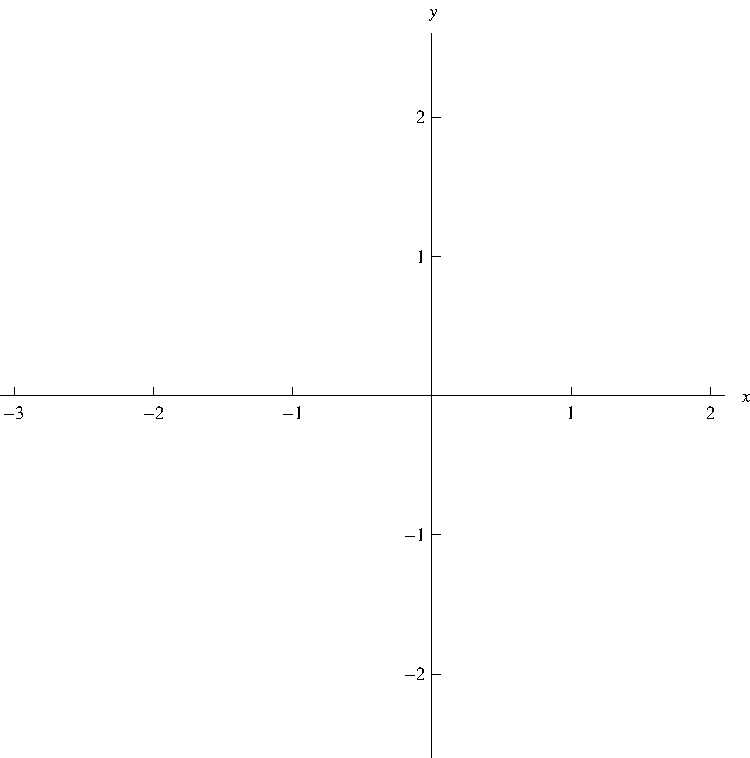
\includegraphics[width=4.5cm]{precalculus/pictures/piecewise-ex2-1.pdf}%
%}%
%\only<9| handout:0>{%
%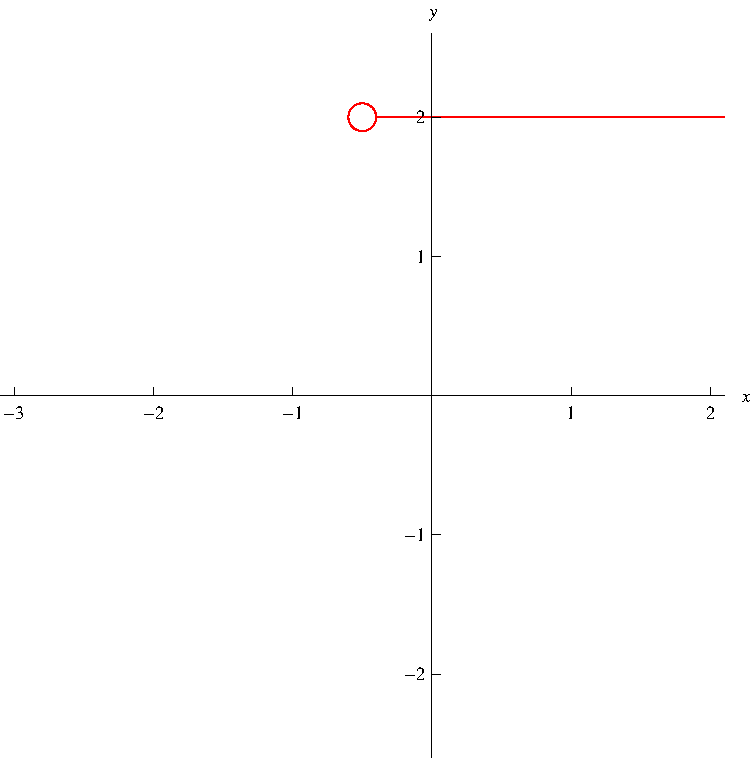
\includegraphics[width=4.5cm]{precalculus/pictures/piecewise-ex2-2.pdf}%
%}%
%\only<10-| handout:1>{%
%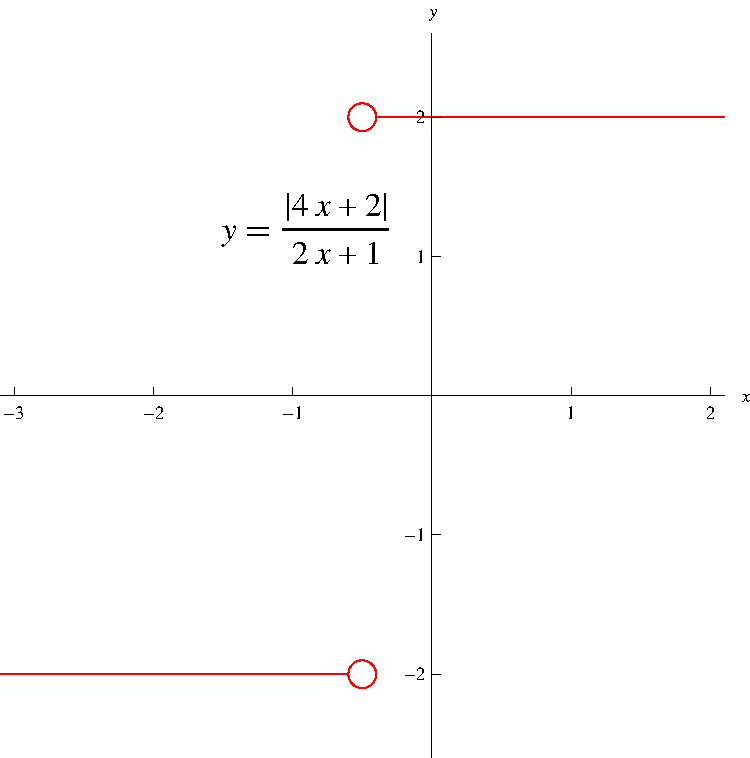
\includegraphics[width=4.5cm]{precalculus/pictures/piecewise-ex2-3.pdf}%
%}%
\column{.55\textwidth}
\abovedisplayskip=0pt
\belowdisplayskip=-15pt
\abovedisplayshortskip=0pt
\belowdisplayshortskip=0pt
\begin{align*}
\uncover<2->{%
|\alert<handout:0| 3>{x}| %
}%
& \uncover<2->{%
 = \begin{cases}
\alert<handout:0| 3>{x} & \text{if $\alert<handout:0| 3>{x} \geq 0$}\\
-\alert<handout:0| 3>{x} & \text{if $\alert<handout:0| 3>{x} < 0$}.\\
\end{cases}
}\\%
\uncover<3->{%
\frac{|\alert<handout:0| 3>{4x+2}|}{2x+1} %
}%
& \uncover<3->{%
 = \begin{cases}
\frac{\alert<handout:0| 3-5>{4x+2}}{2x+1} & \text{if $\alert<handout:0| 3>{4x+2} > 0$}\\
\frac{\alert<handout:0| 6-7>{-(\alert<handout:0| 3>{4x+2})}}{2x+1} & \text{if $\alert<handout:0| 3>{4x+2} < 0$}\\
\end{cases}
}\\%
& \uncover<4->{%
 = \begin{cases}
\frac{\uncover<5->{\alert<handout:0| 5>{2(2x+1)}}}{2x+1} & \text{if $4x > -2$}\\
\frac{\uncover<7->{\alert<handout:0| 7>{-2(2x+1)}}}{2x+1} & \text{if $4x < -2$}\\
\end{cases}
}\\%
& \uncover<8->{%
 = \begin{cases}
\alert<handout:0| 9>{2} & \alert<handout:0| 9>{\text{if $x > -1/2$}}\\
\alert<handout:0| 10>{-2} & \alert<handout:0| 10>{\text{if $x < -1/2$}}.\\
\end{cases}
}%
\end{align*}
\end{columns}
\end{example}
\end{frame}
% end module piecewise-ex2
